\documentclass{article}
\usepackage{graphicx}

\begin{document}

\begin{flushleft}
Contemporary Mathematics\\
Volume 57, 1986
\end{flushleft}







\begin{center}
RECURSIVE ORDERED SETS\\
Henry A. Kierstead
%\maketitle
\end{center}
§ 1 Introduction\\
\indent
Many mathematicians working in finite combinatorics are highly suspicious of infinite sets and structures.   This suspicion does not extend to all infinite structures.   
The set of natural numbers with the usual order is considered quite acceptable and, on the whole, so is the set of real numbers with its usual order.   
The problems arise when some unusual structure is placed on these sets as in well ordering the real numbers.   
Other examples arise from extending theorems about finite structures to theorems about infinite   structures.    
Once Dilworth's Theorem has been proven for finite ordered sets it is routine to extend it to infinite ordered sets of finite width via the Compactness Theorem.   
However the resulting structure may be quite unusual.   
The proof only shows the existence of a chain cover; it does not produce the chain cover.   
This is the source of the uneasiness in both cases:    The structures whose existence is asserted have not been shown to be available for inspection.\\
\indent
Rather than ignoring these existence results one should go one step further and ask whether there is a satisfactory structure available for inspection. 
This leads to further questions. What does it mean to be available for inspection? 
How would you show that there was no satisfactory structure available for inspection? 
For countable structures these concerns can be made precise and can often be resolved using the theory of recursive (i.e. computable) functions.   
The resulting combinatorial theory is the subject of this article, which in particular will'concentrate on antichain covers, chain covers, and realizers of recursive ordered sets.\\
\indent
Let us agree that a structure is available for inspection if it is recursive, where, roughly speaking, a relational structure   P   is recursive if it is recursive, where, roughly speaking, a relational structure P is recursive if\\
\newline
---------------\\
1980 Mathematics Subject Classification. Primary 03D45. supported by ONR grant N00014-85K-0494
\newline

\begin{flushright}
© 1986 American Mathematical Society 0271-4132/86 $1.00 + $.25 per page
\end{flushright}

\newpage

there is a finite algorithm that will provide yes-no answers to questions of the form:  "Is    x    in the domain of    P?" and "Does $\bar{x}$    hold for the relation R?"  We shall see that the uneasiness resulting from the use of the Compactness Theorem is well founded,  for there exist recursive ordered sets (necessarily infinite) with finite width   w   that   cannot be covered by w recursive chains.    
Two reasonable responses to this negative result are the traditional recursion theoretic response of analyzing the "degree of non-computability" of such a cover and the more recent combinatorial response, which we shall pursue, of searching for a recursive chain cover that uses some finite number of additional chains. 
Thus we are asking whether there exists a function b such that every ordered set with fini te width w, which is available for inspection, has a chain cover consisting of b(n) chains, which is available for inspection. 
From a finite point of view this approach leads to a very satisfying theory. 
There can be no doubt that the structures under consideration really exist. 
They are essentially finite since they can be stored using only finitely much space by storing the finite algorithms that describe them.    
They are amenable to the type of explicit construction often used on finite structures.    
The results we prove are quite interrelated. Recursive antichain covers and recursive realizers are used to construct recursive chain covers while recursive chain covers are used to construct recursive realizers.
The proofs rely most heavily on algorithmic techniques and the theory of finite ordered sets.    
Indeed, essentially all the recursion theory needed can be reduced to two lemmas. 
The goal of this article is to present a collection of results, proofs, and problems on recursive ordered sets in a unified setting, which is accessible to discrete mathematicians with little or no background in recursion theory.\\
\newline
For the most part our notation is standard; a few special conventions are mentioned here. The set of natural numbers is represented by n. 
Incomparability in ordered sets is denoted by $\Vert$. The restriction of a structure (a,$\bar{R}$) to the substructure generated by B $\subset$ A is denoted by (a,$\bar{R}$)$\vert$B.\\


§2   K - L   Expansion Theorems\\


In this section we use the language of general relational structures to define the notion of an expansion theorem.   Next we review the basics of elementary recursion theory and present the notion of a recursive expansion theorem.    Finally we introduce expansion games and prove two lemmas which reduce the proofs of recursive expansion theorems to finding winning strategies in expansion games.   These games are interesting in their own right and are related to on line algorithms.

\newpage

A (relational) i \underline{structure} is a system   A = (A, $\bar{R}$)   where   $\bar{R}$   is a sequence of relations on the domain   A.   
To avoid certain technical difficulties we will only consider structures with finitely many relations.    
Structures will be denoted with bold face letters;  the same letter in standard form will denote the domain of the structure.   
Two structures (A,$\bar{R}$)   and   (B,$\bar{S}$) are similar    provided that   $\bar{R}$   and   $\bar{S}$ have    the same length and corresponding entries in   $\bar{R}$   and    $\bar{S}$   have the same rank.    The structure
$(A,R_1,...,R_m...,R_n)$    is an \underline{expansion} of  the structure    $(A,R_1,...,R_m)$.    
Let K be a class of similar structures and let   L   be another class of similar structures.   
A   K - L   \underline{expansion} \underline{theorem} is an assertion of the form: Every structure in   K   has an expansion in   L.    Dilworth's Theorem is an example of a   K - L   expansion theorem. Matching theorems, coloring theorems, and dimension theorems for ordered sets also fall into this category.

There are many equivalent ways to define the concept of a partial recursive or computable function.    
For our purposes it will be enough to say that a \underline{partial} \underline{recursive} \underline{function}  $\Phi$    is a function that can be computed by an algorithm of finite length - if   x   is in the domain of $\Phi$ then the algorithm eventually produces the output $\Phi(x)$ when started on the input   x; if   x is not in the domain of     the algorithm produces no output when started on the input   x.   
A \underline{recursive} \underline{set} is a set whose characteristic function is recursive. 
Notice that every finite set is recursive. A precise definition of these concepts can be found in Machtey and Young [1978].   
The domain of a partial recursive function may not be recursive; if it is we will say that the function is recursive.   
This is a slight variance from the normal definition. 
A structure   A   = (A,$\bar{R}$)    is \underline{recursive} if there is a recursive function  such that both $\Phi(0,x) = 1$   iff   x $\in$ A   and $\Phi(R, \bar{x}) = 1$   iff   $x\in R$, whenever R is in $\bar{R}$. We say that $\Phi$   defines   A.   
If   A   is a recursive structure the domain of   A     and each of its relations are recursive sets.   
To test whether x   is in   A, first check whether   (0,x)   is in the recursive set   dom($\Phi$) and if it is check to see whether   $\Phi(0,x) = 1$.
It is also easy to see that if each of the relations of   A   is recursive and the domain of   A   is recursive then   A   is recursive.   
Thus the domain and each of the relations of a recursive structure are completely described by a single algorithm of finite length. 
A \underline{recursive} K-L \underline{expansion} \underline{theorem} is an assertion of the following form: Every recursive structure in K has can be expanded to a recursive structure in L.\\ 
\indent It is possible to enumerate the countably many possible algorithms. 
Let $\Phi_e$   be the partial recursive function computed by the eth algorithm in such a list.   
The execution of      algorithm on a particular input occurs in a step by step manner.    
If the execution of the   eth   algorithm   on   x   halts after at most   n   steps and outputs   y   we say that   $\Phi_e^n(x)$   is defined and equals y;
\newpage
% SEKCJA Z OBRAZKAMI
\begin{picture}(100, 100)
%\linethickness{2mm}
\thicklines
\put(0, 0){\circle{5}}
\put(0, -40){\circle{5}}
\put(40, 0){\circle{5}}
\put(40, -40){\circle{5}}
\put(2, -38){\line(1, 1){36}}
\put(0, -2){\line(0, -1){36}}
\put(-38, -2){\line(1, 1){36}}
\put(40, -38){\line(0, 1){36}}
\put(40, -38){\line(1, 1){14}}
\put(160, -40){\circle{5}}
\put(160, 0){\circle{5}}
\put(158, -2){\line(-1, -1){14}}
\put(2, -1){\line(4, -1){156}}
\put(160, -2){\line(0, -1){36}}

\put(100, -20){\circle*{3}}
\put(110, -20){\circle*{3}}
\put(120, -20){\circle*{3}}

\end{picture}

\begin{picture}(100, 100)
\thicklines
\put(0, 0){\circle{3}}
\put(0, -20){\circle{3}}
\put(0, -40){\circle{3}}
\put(0, -60){\circle{3}}
\put(0, -80){\circle{3}}
\put(20, -60){\circle{3}}
\put(20, -80){\circle{3}}
\put(40, -60){\circle{3}}
\put(40, -80){\circle{3}}
\put(40, -100){\circle{3}}
\put(40, -120){\circle{3}}
\put(40, -140){\circle{3}}

\put(0, -2){\line(0, -1){16}}
\put(0, -22){\line(0, -1){16}}
\put(0, -42){\line(0, -1){16}}
\put(0, -62){\line(0, -1){16}}
\put(1, -61){\line(1, -1){18}}
\put(1, -79){\line(1, 1){18}}

\put(21, -61){\line(1, -1){18}}
\put(21, -79){\line(1, 1){18}}

\put(40, -62){\line(0, -1){16}}
\put(40, -82){\line(0, -1){16}}
\put(40, -102){\line(0, -1){16}}
\put(40, -122){\line(0, -1){16}}

\put(-15, -1){$c_1^0$}
\put(-15, -61){$c_1^i$}
\put(-20, -81){$c_1^{i+1}$}
\put(24, -58){\footnotesize y}
\put(24, -84){\footnotesize x}
\put(45, -61){$c_2^{i+1}$}
\put(45, -81){$c_2^i$}
\put(45, -141){$c_2^0$}
\put(14, -137){(b)}


\end{picture}

\newpage
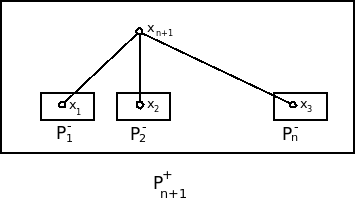
\includegraphics[scale=0.5]{figures/Figure1.png}
\newpage
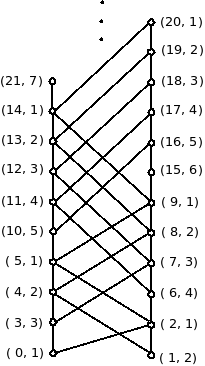
\includegraphics[scale=0.5]{figures/Figure3.png}
\newpage
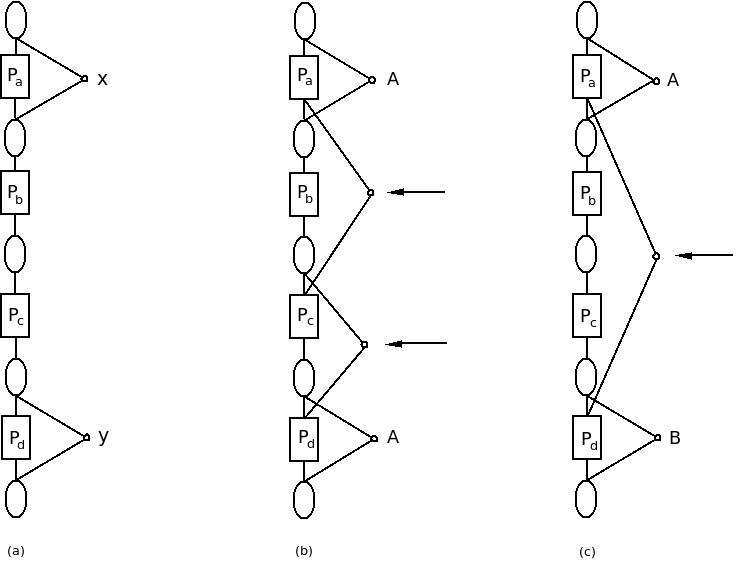
\includegraphics[scale=0.5]{figures/Figure5.png}

\end{document}


